% ============================================================================
%  3. DYNARE EN VIVO  (50--115 min)
% ============================================================================
\section{Dynare}

% S18
\begin{frame}[label=preprocesador]{Dynare traduce, MATLAB ejecuta}
  \centering
  \resizebox{\textwidth}{!}{%
  \begin{tikzpicture}[
    doc/.style={draw=darkblue, thick, fill=white, minimum width=1.7cm, minimum height=2.1cm,
      align=center, font=\small},
    fil/.style={draw=errframe!70, fill=errframe!8, rounded corners=1pt, font=\ttfamily\small,
      text width=3.5cm, inner sep=2.5pt, align=center},
    res/.style={draw=darkblue, fill=thmblue, rounded corners=2pt, font=\ttfamily\small,
      minimum width=1.7cm, inner sep=3pt},
    go/.style={-{Stealth[length=2.3mm]}, very thick, darkblue}]
    \node[doc] (mod) at (-0.6,0) {\ttfamily rbc\_\\\ttfamily taller\\\ttfamily .mod};
    \node[fil] (f1) at (4.6,0.9) {driver.m};
    \node[fil] (f2) at (4.6,0.3) {static\_resid.m, \ldots};
    \node[fil] (f3) at (4.6,-0.3) {dynamic\_g1.m, \ldots};
    \node[fil] (f4) at (4.6,-0.9) {steadystate.m};
    \node[res] (M) at (8.6,0.8) {M\_};
    \node[res] (op) at (8.6,0) {options\_};
    \node[res] (oo) at (8.6,-0.8) {oo\_};
    \begin{scope}[on background layer]
      \node[draw=darkblue, very thick, rounded corners=6pt, fill=thmblue!35,
        fit=(f1)(f4)(M)(oo), inner xsep=9pt, inner ysep=11pt] (mat) {};
    \end{scope}
    \node[font=\bfseries\small, text=darkblue, anchor=south] at (mat.north) {MATLAB};
    \draw[go] (mod.east) -- node[above=2pt, font=\footnotesize, align=center]{pre-\\procesador} (mod.east -| mat.west);
    \draw[go] ($(f2.east)!0.5!(f3.east)+(0.1,0)$) -- ($(op.west)+(-0.1,0)$);
    \node[font=\footnotesize\itshape, text=darkblue] at (-0.6,-1.6) {lo que escribes};
    \node[font=\footnotesize\itshape, text=darkblue] at (4.6,-1.8) {lo que genera Dynare};
    \node[font=\footnotesize\itshape, text=darkblue] at (8.6,-1.8) {resultados};
  \end{tikzpicture}}
  \par\vspace{0.5cm}\raggedright
  \texttt{dynare rbc\_taller} lee el \texttt{.mod}, comprueba la sintaxis, calcula las
  derivadas \textbf{analíticamente} y escribe archivos de MATLAB.\par
  \vspace{0.25cm}
  Los resultados quedan en tres estructuras: \cod{M\_} (el modelo), \cod{options\_}
  (las opciones) y \cod{oo\_} (los resultados).
  \fuente{Inspirada en \textcite[Fig.~2.1]{gmo}.}
\end{frame}

% S19
\begin{frame}[fragile,label=arranque]{Antes de escribir una línea}
  \begin{lstlisting}[language={}]
>> addpath C:\dynare\7.1\matlab     % una vez por sesion
>> cd <carpeta del taller>
>> edit rbc_taller.mod              % abre el archivo
\end{lstlisting}
  \vspace{0.3cm}
  El archivo tiene \textbf{20 huecos} \texttt{???}, numerados \texttt{[H1]} a
  \texttt{[H20]}, ordenados según los cinco bloques de un \texttt{.mod}.\par
  \vspace{0.3cm}
  Cada hueco trae una pista y la sección del handout que lo explica.\par
  \vspace{0.3cm}
  Dynare no corre mientras quede un \texttt{???} activo. Si lo intentas:
  \begin{lstlisting}[language={}]
ERROR: rbc_taller.mod: line 37, col 5: character
       unrecognized by lexer
\end{lstlisting}
  \note{Que todos corran el archivo sin tocarlo y vean este error: así lo reconocen
  después. La línea 37 es el hueco H1.}
\end{frame}

% S20
\begin{frame}[label=bloques]{Los cinco bloques de un \texttt{.mod}}
  \centering
  \renewcommand{\arraystretch}{1.45}
  \begin{tabular}{@{}cl>{\raggedright\arraybackslash}p{4.4cm}c@{}}
    \toprule
    & \textbf{Bloque} & \textbf{Qué contiene} & \textbf{Huecos}\\
    \midrule
    1 & Preámbulo & \texttt{var}, \texttt{varexo}, \texttt{parameters} y calibración & H1--H7\\
    2 & Modelo & las ocho ecuaciones & H8--H15\\
    3 & Estado estacionario & \texttt{steady\_state\_model} & H16--H17\\
    4 & Choques & \texttt{shocks} & H18\\
    5 & Cálculo & \texttt{steady}, \texttt{check}, \texttt{stoch\_simul} & H19--H20\\
    \bottomrule
  \end{tabular}
  \par\vspace{0.4cm}\raggedright
  El orden no es arbitrario: es el orden en que Dynare necesita la información.
  \fuente{Handout, §3.2. Inspirada en \textcite[Fig.~2.2]{gmo}.}
\end{frame}

% S21
\begin{frame}[fragile,label=etapa1]{Etapa 1: el preámbulo}
  \begin{lstlisting}
var y c i k h r w a;      // [H1] 8 endogenas
varexo eps;               // [H2] el choque
parameters alpha beta delta phi sigma_eps theta hss
           r_ss k_ss y_ss i_ss c_ss w_ss;
alpha = 0.667;            // ... calibracion
r_ss  = ???;              // [H3]  (lamina ee)
k_ss  = ???;              // [H4]
theta = ???;              // [H7]
\end{lstlisting}
  \vspace{0.2cm}
  Un parámetro puede definirse a partir de otros ya asignados: así calculamos el estado
  estacionario cerrado sin resolver nada.\par
  \vspace{0.25cm}
  \textbf{10 minutos.} Completa H1--H7 con la lámina del estado estacionario.
  \note{Respuestas en el solucionario. Error típico en H4: usar $\alpha$ como
  participación del capital.}
\end{frame}

% S22
\begin{frame}[label=reglas]{Etapa 2: cómo se escribe una ecuación}
  \begin{enumerate}
    \item Una ecuación por línea, terminada en \texttt{;}.\par\vspace{0.12cm}
    \item El tiempo va entre paréntesis: \texttt{c(+1)} es $c_{t+1}$ y \texttt{k(-1)} es
      $k_{t-1}$.\par\vspace{0.12cm}
    \item No se escribe $\mathbb{E}_t$: todo \texttt{(+1)} está en esperanza.\par\vspace{0.12cm}
    \item Operaciones como en MATLAB: \texttt{*}, \texttt{/}, \texttt{\^{}},
      \texttt{log()}, \texttt{exp()}.\par\vspace{0.12cm}
    \item Una etiqueta \texttt{[name='Euler']} antes de la ecuación ayuda a leer los
      errores.
  \end{enumerate}
  \vspace{0.3cm}
  \begin{block}{La regla que más errores evita}
    Cada variable se fecha por el período en que \textbf{se decide}.
  \end{block}
\end{frame}

% S23
\begin{frame}[label=timing]{El timing del capital}
  \centering
  \begin{tikzpicture}[font=\small, >={Stealth[length=2mm]}]
    \draw[thick, ->] (0,0) -- (10,0) node[right]{$t$};
    \foreach \x/\l in {1.5/{$t-1$}, 5/{$t$}, 8.5/{$t+1$}}{
      \draw[thick] (\x,0.12) -- (\x,-0.12) node[below]{\l};}
    \draw[very thick, darkblue, ->] (1.6,0.35) to[bend left=30]
      node[above, align=center]{se elige en $t-1$,\\ se usa en $t$} (4.9,0.35);
    \node[draw=darkblue, fill=thmblue, rounded corners=2pt, align=center] at (3.25,-1.35)
      {Pizarra: $k_t$\\ Dynare: \texttt{k(-1)}};
    \draw[very thick, errframe, ->] (5.1,0.35) to[bend left=30]
      node[above, align=center]{se elige en $t$,\\ se usa en $t+1$} (8.4,0.35);
    \node[draw=errframe, fill=errframe!8, rounded corners=2pt, align=center] at (6.75,-1.35)
      {Pizarra: $k_{t+1}$\\ Dynare: \texttt{k}};
  \end{tikzpicture}
  \par\vspace{0.4cm}\raggedright
  En Dynare, \texttt{k} es el capital elegido \emph{hoy}. El que produce hoy es
  \texttt{k(-1)}.\par
  \vspace{0.2cm}
  Producción y demanda de capital deben usar \texttt{k(-1)}; la ley de movimiento
  escribe \texttt{k} a la izquierda.
  \fuente{Handout, §3.2.2.}
  \note{Es el error número uno. Preguntar: en la ley de movimiento, ¿qué capital va a la
  izquierda?}
\end{frame}

% S24
\begin{frame}[label=etapa2]{Etapa 2: del papel al código}
  \centering\small
  \renewcommand{\arraystretch}{1.4}
  \begin{tabular}{@{}cll@{}}
    \toprule
    \textbf{Hueco} & \textbf{Papel} & \textbf{Pista}\\
    \midrule
    H8 & $1/c_t=\beta\,\mathbb{E}_t[(r_{t+1}+1-\delta)/c_{t+1}]$ & retorno de mañana\\
    H9 & $\theta c_t/(1-h_t)=w_t$ & \\
    H10 & $r_t=(1-\alpha)y_t/k_{t-1}$ & timing\\
    H11 & $w_t=\alpha y_t/h_t$ & \\
    H12 & $y_t=a_tk_{t-1}^{1-\alpha}h_t^{\alpha}$ & timing\\
    H13 & $k_t=(1-\delta)k_{t-1}+i_t$ & \\
    H14 & $y_t=c_t+i_t$ & \\
    H15 & $\ln a_t=\phi\ln a_{t-1}+\sigma_\varepsilon\varepsilon_t$ & en logaritmos\\
    \bottomrule
  \end{tabular}
  \par\vspace{0.35cm}\raggedright
  \textbf{15 minutos.} Escribe las ocho ecuaciones en el bloque \texttt{model}.
  \note{Caminar por el aula. Revisar H8 (r(+1)), H10 y H12 (k(-1)) en cada pantalla.}
\end{frame}

% S25
\begin{frame}[fragile,label=etapa2-sol]{Etapa 2 resuelta}
  \begin{lstlisting}
model;
  1/c = beta*(1/c(+1))*(r(+1) + 1 - delta);   // H8
  theta*c/(1 - h) = w;                        // H9
  r = (1 - alpha)*y/k(-1);                    // H10
  w = alpha*y/h;                              // H11
  y = a*k(-1)^(1 - alpha)*h^alpha;            // H12
  k = (1 - delta)*k(-1) + i;                  // H13
  y = c + i;                                  // H14
  log(a) = phi*log(a(-1)) + sigma_eps*eps;    // H15
end;
\end{lstlisting}
  \vspace{0.2cm}
  Ocho ecuaciones, casi idénticas a la pizarra. La única traducción real es el
  \textbf{timing}.
  \note{Mostrar solo después de que la mayoría haya intentado. Las etiquetas
  [name=...] se omiten aquí por espacio; en el archivo están.}
\end{frame}

% S26
\begin{frame}[fragile,label=etapa34]{Etapas 3 y 4: estado estacionario y choque}
  \begin{lstlisting}
steady_state_model;
  a = ???;               // [H16]  ojo: a, no ln a
  r = r_ss;  h = hss;
  k = ???;  y = ???;  i = ???;  c = ???;  w = ???;  // [H17]
end;

shocks;
  var eps; stderr ???;   // [H18]
end;
\end{lstlisting}
  \vspace{0.2cm}
  \texttt{steady\_state\_model} no resuelve nada: solo \textbf{evalúa} las fórmulas
  cerradas del preámbulo.\par
  \vspace{0.25cm}
  ¿Por qué \texttt{stderr} no debería ser $0.0072$?
  \note{H16 = 1 (ln 1 = 0; con 0, log(0) no existe). H18 = 1: sigma\_eps ya escala el
  choque dentro de la PTF; con 0.0072 el choque queda escalado dos veces y las IRF salen
  139 veces más chicas.}
\end{frame}

% S27
\begin{frame}[fragile,label=control1]{Punto de control 1: \texttt{steady} y \texttt{resid}}
  \begin{lstlisting}[language={}]
>> dynare rbc_taller
\end{lstlisting}
  \vspace{0.1cm}
  \centering\small
  \texttt{STEADY-STATE RESULTS}\par\vspace{0.1cm}
  \begin{tabular}{@{}cccccccc@{}}
    \toprule
    $y$ & $c$ & $i$ & $k$ & $h$ & $r$ & $w$ & $a$\\
    \midrule
    0.5673 & 0.4528 & 0.1145 & 4.5785 & 0.2000 & 0.0413 & 1.8919 & 1.0000\\
    \bottomrule
  \end{tabular}
  \par\vspace{0.35cm}\raggedright\normalsize
  Los ocho residuos deben salir en \texttt{0.000000}.\par
  \vspace{0.2cm}
  Escribe \texttt{theta} en la ventana de comandos: \num{3.3424}.\par
  \vspace{0.3cm}
  \begin{block}{Si un residuo no es cero}
    Hay un error de álgebra en el estado estacionario. La ecuación con residuo es la
    sospechosa.
  \end{block}
  \note{Un residuo cero no garantiza que el modelo esté bien: si en H13 alguien escribió
  k = (1-delta)*k + i, el estado estacionario cuadra igual. Lo delata el control 3.}
\end{frame}

% S28
\begin{frame}[fragile,label=control2]{Punto de control 2: \texttt{check} (H19)}
  \begin{lstlisting}[language={}]
EIGENVALUES:
   Modulus      Real   Imaginary
     0.936     0.936           0
     0.979     0.979           0
     1.086     1.086           0
 1.145e+18 1.145e+18           0
There are 2 eigenvalue(s) larger than 1 in modulus
for 2 forward-looking variable(s).
The order and rank conditions are verified.
\end{lstlisting}
  \vspace{0.15cm}
  $0.936$, $0.979$ y $1.086$: los de la pizarra.\par
  \vspace{0.15cm}
  ¿Y el gigante? \texttt{r} aparece como \texttt{r(+1)} en la Euler, así que Dynare la
  cuenta como variable que salta. Es estática: su valor propio es infinito. Dos raíces
  inestables para dos \emph{jumpers}.
  \note{La economía es la misma: un solo salto genuino, el consumo. Si sustituimos r en la
  Euler, el valor propio infinito desaparece.}
\end{frame}

% S29
\begin{frame}[label=control3]{Punto de control 3: la regla de decisión (H20)}
  \centering\small
  \texttt{stoch\_simul(order = 1, irf = 40) y c i k h r w a;}\par
  \vspace{0.25cm}
  \setlength{\tabcolsep}{4.5pt}
  \begin{tabular}{@{}lrrrrr@{}}
    \toprule
    & $y$ & $c$ & $i$ & $k$ & $h$\\
    \midrule
    Constante & 0.5673 & 0.4528 & 0.1145 & 4.5785 & 0.2000\\
    \texttt{k(-1)} & 0.0134 & 0.0524 & $-0.0390$ & \num{0.9360} & $-0.0147$\\
    \texttt{a(-1)} & 0.8205 & 0.2584 & 0.5621 & 0.5621 & 0.1401\\
    \texttt{eps} & 0.0060 & 0.0019 & 0.0041 & 0.0041 & 0.0010\\
    \bottomrule
  \end{tabular}
  \par\vspace{0.3cm}\raggedright\normalsize
  Está en \textbf{niveles}: cada número es una desviación del estado estacionario.\par
  \vspace{0.15cm}
  La diagonal lleva el valor propio estable: el capital de hoy hereda $0.936$ del de
  ayer.\par
  \vspace{0.15cm}
  En elasticidad: $0.0524\times k_{ss}/c_{ss}=0.0524\times4.5785/0.4528=\num{0.530}$.
  \note{La fila eps es la del impacto: el primer punto de cada IRF. Es la fila a(-1)
  multiplicada por sigma/phi.}
\end{frame}

% S30
\begin{frame}[label=errores]{Lo que va a fallar}
  \footnotesize
  \renewcommand{\arraystretch}{1.2}
  \begin{tabular}{@{}>{\raggedright\arraybackslash}p{4.6cm}>{\raggedright\arraybackslash}p{5.6cm}@{}}
    \toprule
    \textbf{Síntoma} & \textbf{Causa probable}\\
    \midrule
    \texttt{character unrecognized by lexer} & queda un \texttt{???}\\
    Símbolo no declarado & falta en \texttt{var} o \texttt{parameters}\\
    Residuo distinto de cero & error en el estado estacionario\\
    Residuos no finitos & \texttt{a = 0} en \texttt{steady\_state\_model}: $\ln 0$\\
    \texttt{Blanchard \& Kahn conditions are not satisfied} & timing: \texttt{k(+1)} o \texttt{k} donde va \texttt{k(-1)}\\
    IRF 139 veces más chicas & \texttt{stderr 0.0072}: choque escalado dos veces\\
    Términos de segundo orden & falta \texttt{order = 1}: el valor por defecto es 2\\
    \bottomrule
  \end{tabular}
  \fuente{Handout, §3.13, ``Depuración''.}
  \note{El comando que se detiene localiza la avería: steady, resid, check, stoch\_simul,
  en ese orden.}
\end{frame}

% S31
\begin{frame}[label=donde-guarda]{Dónde quedan los resultados}
  \small
  \cod{oo\_.steady\_state}: estado estacionario.\par
  \cod{oo\_.irfs.c\_eps}: IRF del consumo, en niveles.\par
  \cod{oo\_.dr.ghx}, \cod{oo\_.dr.ghu}: regla de decisión.\par
  \vspace{0.15cm}
  \centering
  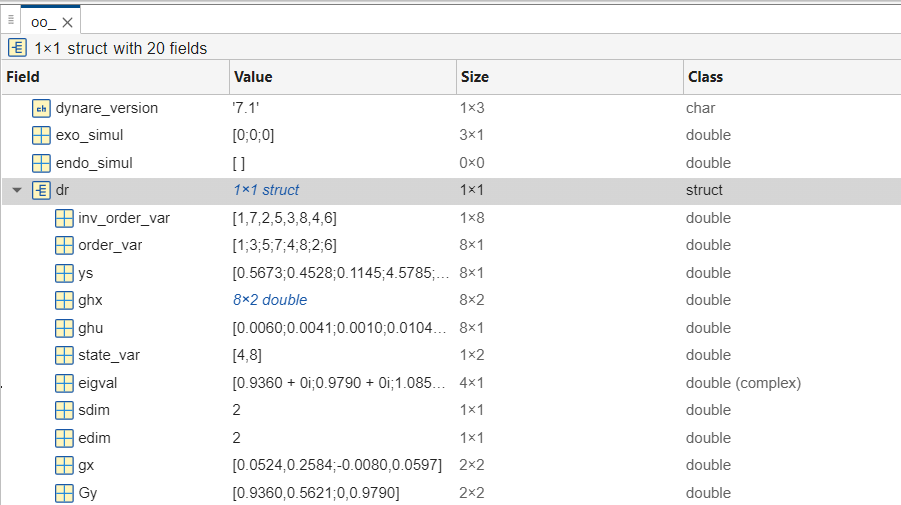
\includegraphics[width=0.72\textwidth]{04_oo_dr.png}\par
  \vspace{0.1cm}\raggedright
  \textbf{Trampa:} las filas de \texttt{ghx} siguen el \emph{orden DR}
  (\texttt{order\_var}), no el de \texttt{var}. La fila 2 es $i$, no $c$.\normalsize
  \fuente{Handout, §3.7. Captura de MATLAB con Dynare 7.1.}
  \note{\texttt{reconstruir\_irf.m} rearma las IRF desde ghx y ghu; coincide con
  oo\_.irfs hasta 4e-16.}
\end{frame}

% S32
{
\setbeamercolor{background canvas}{bg=UWBlack}
\begin{frame}[label=pausa]
  \centering\vfill
  {\color{UWGoldL3}\fontsize{28}{32}\selectfont\bfseries Pausa\par}
  \vspace{0.4cm}
  {\color{UWWhite}\large 10 minutos\par}
  \vspace{0.6cm}
  {\color{UWGrayL2}\small Al volver: ¿qué hace la economía con esos números?\par}
  \vfill
\end{frame}
}
